\section{The degree-two versus degree-three dichotomy}\label{deg:sec:degree}
In this section the host is simple and unweighted, and one existing edge
is doubled. The updated edge has conductance two. Write
$W_{\mathrm{path},\alpha}(\varepsilon)$ for the supremal strict count over
all paths and edge locations, and $W_{d,\alpha}(\varepsilon)$ for that
supremum over connected hosts of maximum degree at most $d$.
The combinatorial degree does not change when an edge is doubled.
Write $C_\alpha=C=\mathcal C_\alpha(L,L')$ for this graph response.

\begin{theorem}[Sharp degree laws]\label{deg:thm:main}
For each fixed $0<\alpha<1$, as $\varepsilon\downarrow0$,
\[
 W_{\mathrm{path},\alpha}(\varepsilon)
 \sim W_{2,\alpha}(\varepsilon)
 \sim\frac1{2\pi^2}\log^2(1/\varepsilon).
\]
For every fixed integer $d\ge3$,
\[
 \lim_{\varepsilon\downarrow0}\varepsilon W_{d,\alpha}(\varepsilon)
 =A_{d,\alpha}:=\alpha\log\frac{2d}{d+2}.
\]
The same higher-degree coefficient is obtained by restricting to
bipartite hosts and bridge edits. These lower examples have leverage
exactly one. The sharp higher-degree assertion is proved in
Theorem~\ref{sharp:thm:sharp} below. The degree-two coefficient is
independent of the fixed exponent $\alpha$.
\end{theorem}

The strict count is precisely the minimum rank needed to approximate
the positive relative matrix in operator norm to tolerance
$\varepsilon$. A positive spectral truncation corresponds to
$0\preceq (L'^\alpha-L^\alpha)-F\preceq\varepsilon L^\alpha$
on the common support. These are structural existence results;
no running-time or finite-precision bound is asserted.

\subsection{Resolvents, leverage measure, and the uniform degree-two upper}
For $A\succ0$, $B=A+uu^T$, set $\tau=u^TA^{-1}u$ and
$c_\alpha=\sin(\pi\alpha)/\pi$. Sherman--Morrison and the scalar
fractional resolvent integral give
\begin{equation}\label{deg:eq:res}
 C=c_\alpha\int_0^\infty
 \frac{t^\alpha v_tv_t^T}{1+m(t)}\,dt,\quad
 v_t=A^{-\alpha/2}(A+tI)^{-1}u,\quad
 m(t)=u^T(A+tI)^{-1}u.
\end{equation}
Write $H$ for the same integral without its denominator. Since
$0\le m(t)\le\tau$,
\begin{equation}\label{deg:eq:sandwich}
 (1+\tau)^{-1}H\preceq C\preceq H.
\end{equation}
In an eigenbasis $A\phi_k=\lambda_k\phi_k$, put
$z_k=|\langle u,\phi_k\rangle|^2/\lambda_k$ and
$\nu=\sum_kz_k\delta_{\lambda_k}$. Then
\begin{equation}\label{deg:eq:diag}
 H_{kk}=\alpha z_k,\qquad
 \tr(1_{(0,\delta]}(A)C1_{(0,\delta]}(A))
                                      \le\alpha\nu((0,\delta]).
\end{equation}
The diagonal identity follows by differentiating the scalar power
integral. Also, after diagonal sign conjugation,
\begin{equation}\label{deg:eq:kernel}
 H_{ij}=\sqrt{z_iz_j}K_\alpha(\log\lambda_i-\log\lambda_j),\qquad
 K_\alpha(s)=\frac{\sinh(\alpha s/2)}{\sinh(s/2)},\quad K_\alpha(0)=\alpha.
\end{equation}

With convention $\widehat K(\xi)=\int e^{-i\xi s}K(s)\,ds$, the beta
integral, equivalently NIST DLMF Table~1.14.1~\cite{DLMF}, gives
\begin{equation}\label{deg:eq:symbol}
 \widehat K_\alpha(\xi)=
 \frac{2\pi\sin(\pi\alpha)}{\cosh(2\pi\xi)+\cos(\pi\alpha)}.
\end{equation}


\begin{lemma}[Exact unit-path measure]\label{deg:lem:pathmeasure}
On the path with $n$ vertices, for the edge $(p,p+1)$,
\[
 \lambda_k=4\sin^2\frac{k\pi}{2n},\qquad
 z_k=\frac2n\sin^2\frac{k\pi p}{n},\quad 1\le k<n.
\]
In particular $\nu((0,\delta])\le\sqrt\delta$, uniformly in $n,p$.
On the cycle with $n\ge3$ vertices, the complex Fourier eigenbasis gives
$\lambda_k=4\sin^2(\pi k/n)$ and $z_k=1/n$, $1\le k<n$;
there $\nu((0,\delta])\le\sqrt\delta/2$.
\end{lemma}
\begin{proof}
The normalized nonconstant path eigenvectors are
$\phi_k(j)=\sqrt{2/n}\cos(k\pi(j-1/2)/n)$.
Subtract their values across the edge and divide the squared difference
by $\lambda_k$. Since $\sin x\ge2x/\pi$ for $0\le x\le\pi/2$,
$\lambda_k\ge4k^2/n^2$. Thus at most $n\sqrt\delta/2$
positive eigenvalues are at most $\delta$, each having leverage weight
at most $2/n$. On a cycle,
$|b^T\phi_k|^2=\lambda_k/n$ and
$\lambda_k\ge16\min(k,n-k)^2/n^2$; counting both ends of the
Fourier grid proves the stated bound. Complex eigenvectors merely
diagonalize a real self-adjoint operator and do not change its spectrum.
\end{proof}

\begin{lemma}[Positive pinching]\label{deg:lem:pinch}
For complementary orthogonal projections $P,Q$ and $C\succeq0$,
$C\preceq2(PCP+QCQ)$. In particular, if
$\|QCQ\|\le\varepsilon/2$, then
$\N_C(\varepsilon)\le\N_{PCP}(\varepsilon/2)$.
\end{lemma}
\begin{proof}
Apply $2\langle C^{1/2}Px,C^{1/2}Qx\rangle
\le\|C^{1/2}Px\|^2+\|C^{1/2}Qx\|^2$.
The upper bound is block diagonal; its $Q$ block has no eigenvalue
strictly greater than $\varepsilon$.
\end{proof}

\subsubsection{One fixed continuum operator controls every finite grid}
\begin{lemma}[Uniform Cauchy-cell comparison]\label{deg:lem:cell-grid}
Fix $0<\alpha<1$, let $a=\sqrt2$, and let $S$ be the positive integral
operator on $L^2(0,a)$ with kernel $\sqrt{xy}/(x+y)$.
Suppose $x_1,\ldots,x_N\in(0,2]$ and $h>0$ satisfy $hN\le1$.
For all low nodes $x_i\le a$, suppose $x_i\ge2h$ and the intervals
$I_i=[x_i-h,x_i]$ are pairwise disjoint. Put
\[
 T_{\alpha,h}(i,j)=hK_\alpha(\log x_i^2-\log x_j^2),\qquad
 M_\alpha=\max\{\sin(\pi\alpha),\tan(\pi\alpha/2)\}.
\]
Uniformly over all such finite grids,
\[
 \N_{T_{\alpha,h}}(\varepsilon)
 \le\N_S\!\left(\frac{\varepsilon}{4M_\alpha\log2}\right)
       +O_\alpha(1+\log^+(1/\varepsilon)),
 \qquad \log^+t=\max(0,\log t).
\]
Consequently their uniform upper count coefficient is at most
$1/(2\pi^2)$ at scale $\log^2(1/\varepsilon)$.
\end{lemma}
\begin{proof}
The ratio of the Fourier symbol in~\eqref{deg:eq:symbol} to its value
at $\alpha=1/2$ is
\[
 \frac{\sin(\pi\alpha)\cosh(2\pi\xi)}
      {\cosh(2\pi\xi)+\cos(\pi\alpha)}\le M_\alpha.
\]
Fourier inversion gives, on every finite real grid $t_i$,
\[
 \sum_{i,j}\overline v_i v_jK_\alpha(t_i-t_j)
  =\frac1{2\pi}\int_{\R}\widehat K_\alpha(\xi)
                   \left|\sum_jv_je^{i\xi t_j}\right|^2d\xi.
\]
Thus $T_{\alpha,h}\preceq M_\alpha T_{1/2,h}$ in Loewner order,
including for atomic grids. It suffices to consider $\alpha=1/2$, when
\[
 T_{1/2,h}(i,j)=h\frac{\sqrt{x_ix_j}}{x_i+x_j}.
\]

For each low node define
\[
 f_i(x)=\frac{\sqrt{x_i}}{\sqrt h\sqrt x}\,1_{I_i}(x).
\]
These functions are orthogonal, and
\[
 d_i^2=\norm{f_i}^2
   =\frac{x_i}{h}\log\frac{x_i}{x_i-h}\le2\log2.
\]
Indeed $r\log(r/(r-1))$ decreases for $r>1$, and $x_i/h\ge2$.
The Laplace formula for $(x+y)^{-1}$ shows that $S$ is positive and
trace class, with trace $a/2$. Its compressed Gram matrix is
\[
 B_{ij}=\langle f_i,Sf_j\rangle
 =h\sqrt{x_ix_j}\int_0^\infty e^{-t(x_i+x_j)}\phi(ht)^2dt,
 \qquad \phi(z)=\frac{e^z-1}{z},\quad\phi(0)=1.
\]
Every cell has the same length, so the multiplier is common to all
coordinates. Since $\phi(z)\ge1$ for $z\ge0$,
\[
 v^*(B-T_{\rm low})v
 =h\int_0^\infty[\phi(ht)^2-1]
       \left|\sum_i v_i\sqrt{x_i}e^{-tx_i}\right|^2dt\ge0.
\]
The integrals converge because $x_i\ge2h$. This is a positive
quadratic-form comparison, rather than an entrywise inference.
Normalize $f_i/d_i$ to obtain an isometry $J$ and write
$B=D J^*SJ D$, $D=\diag(d_i)$.
Compression min--max and the singular values of $S^{1/2}JD$ give
\[
 \lambda_j(T_{\rm low})\le\lambda_j(B)
                \le2\log2\,\lambda_j(S).
\]
No Loewner inequality $DTD\preceq\norm D^2T$ is used.

On the high block $a<x_i\le2$, expand
\[
 \frac1{x+y}=\sum_{\ell=0}^{q-1}
       \frac{(-1)^\ell(x-a)^\ell}{(a+y)^{\ell+1}}+R_q(x,y),
 \qquad |R_q(x,y)|\le\frac{r_0^q}{2a},\quad
 r_0=\frac{2-a}{2a}<1.
\]
After multiplication by $h\sqrt{xy}$ this is a rank-$q$ matrix
approximation whose entry errors are at most $hr_0^q/a$.
Since the block has at most $N$ rows and $hN\le1$, its operator error
is at most $r_0^q/a$. The best-rank singular-value bound, also valid
for this possibly nonsymmetric approximant, gives
\[
 \N_{T_{\rm high}}(t)=O(1+\log^+(1/t)).
\]
Positive pinching, Lemma~\ref{deg:lem:pinch}, bounds the full count by
the sum of the two block counts at half the threshold. This proves the
displayed estimate, first at $\alpha=1/2$ and then for every fixed
$\alpha$ by the Fourier comparison.

Laptev's classical weighted-Cauchy theorem~\cite[Theorem (3)]{Laptev}
with exponent one and weights $x^{1/2}y^{1/2}$ has parameter
$\rho=1$ and gives
\[
 \N_S(\varepsilon)\sim\frac1{2\pi^2}\log^2(1/\varepsilon).
\]
Rescaling $(0,1)$ to $(0,a)$ only multiplies eigenvalues by a fixed
factor. The symmetric exponent-one case is explicitly attributed by
Laptev to Widom's earlier Hankel theorem. Crucially, $S$ is fixed before
taking the supremum over grids. Constant threshold factors and the
uniform logarithmic remainder do not change its leading coefficient.
\end{proof}

\begin{proof}[Sharp uniform upper in Theorem~\ref{deg:thm:main}]
For a path on $n$ vertices set
\[
 h=1/n,\qquad x_k=2\sin(k\pi/(2n)),\quad1\le k<n.
\]
The low nodes have $k\le\lfloor n/2\rfloor$, $x_1\ge2h$, and
successive spacing at least $\pi/(\sqrt2n)>2h$.
Their left cells satisfy Lemma~\ref{deg:lem:cell-grid}; also
$h(n-1)\le1$. The derivative in~\eqref{deg:eq:kernel} is
$R T_{\alpha,h}R$, with $R_{kk}=\sqrt{nz_k}$ and $\norm R^2\le2$.
The sandwich~\eqref{deg:eq:sandwich} and bounded-congruence eigenvalue
comparison give $\lambda_j(C)\le2\lambda_j(T_{\alpha,h})$.
Hence the upper coefficient is at most $1/(2\pi^2)$, uniformly over
all path sizes and all edited locations.

For a cycle on $n\ge3$ vertices, combine each equal eigenvalue pair
$\lambda_k=\lambda_{n-k}$ into its one active incidence coordinate.
Its leverage weight is $2/n$; if $n$ is even, the singleton
$\lambda_{n/2}=4$ has weight $1/n$.
Set
\[
 h=2/n,\qquad x_k=2\sin(\pi k/n),\quad
                       1\le k\le\lfloor n/2\rfloor.
\]
Now $h\lfloor n/2\rfloor\le1$. Low nodes have
$k\le\lfloor n/4\rfloor$, $x_1\ge4/n=2h$ whenever this set is nonempty,
and spacing at least $\sqrt2\pi/n>2h$.
Thus the same lemma applies, including when the low set is empty.
The active derivative is a diagonal congruence of $T_{\alpha,h}$
with norm at most one; its even endpoint factor is $1/\sqrt2$.
All other incidence coordinates have zero response.
The same uniform upper coefficient therefore holds over all cycles.
Every connected simple graph of maximum degree two with an edge is a
path or cycle. The centered-path lower bound below matches this uniform
upper for both $W_{\mathrm{path},\alpha}$ and $W_{2,\alpha}$.
\end{proof}

\begin{remark}
A nonsharp logarithmic-squared upper can alternatively be obtained from
low-energy leverage truncation, Stahl's root-exponential rational
approximation~\cite{Stahl}, and the classical rational update rank
identity discussed in~\cite[Section 3.3]{BCKS}.
The equal-width cell argument proves the sharp coefficient without
assuming a uniform finite-grid Nystr\"om convergence rate.
\end{remark}


\subsection{A matching lower bound from the centered-path limit}
Let $C_N$ be the correction for the central edge of the path on $2N$
vertices. In Lemma~\ref{deg:lem:pathmeasure}, exactly the odd indices
contribute, each with weight $1/N$. Their leverage measures converge to
\begin{equation}\label{deg:eq:arcsine}
 d\nu(\lambda)=\frac{d\lambda}{\pi\sqrt{\lambda(4-\lambda)}},\quad
 0<\lambda<4,
\end{equation}
which is uniform $d\theta/\pi$ under
$\lambda=4\sin^2(\theta/2)$, $0<\theta<\pi$.

\begin{theorem}[Exact centered-limit count]\label{deg:thm:center}
After isometric embeddings of their cyclic supports, $C_N$ converge
in Hilbert--Schmidt norm to a positive compact operator $C_\infty$,
and
\[
 \N_{C_\infty}(\varepsilon)
             \sim\frac1{2\pi^2}\log^2(1/\varepsilon).
\]
The constant is independent of fixed $0<\alpha<1$.
\end{theorem}
\begin{proof}
The limiting derivative is the integral operator on $L^2(\nu)$ with
kernel $K_\alpha(\log\lambda-\log\eta)$.
Identify the finite cyclic space with normalized step functions on the
$N$ equal cells in $(0,\pi)$; the contributing angles are the cell
midpoints. The embedded derivative kernels converge pointwise almost
everywhere and are bounded by $\alpha$. Thus they converge in
Hilbert--Schmidt norm.

The exact kernels on $L^2(\nu_N)$ are
\[
 F_N(\lambda,\eta)=c_\alpha(\lambda\eta)^{(1-\alpha)/2}
 \int_0^\infty\frac{t^\alpha\,dt}
 {(\lambda+t)(\eta+t)(1+m_N(t))},\quad
 m_N(t)=\int\frac{\lambda}{\lambda+t}\,d\nu_N(\lambda).
\]
For $t>0$, midpoint quadrature gives
$m_N(t)\to1-\sqrt{t/(t+4)}$.
At every positive $\lambda,\eta$, dominated convergence in $t$
gives convergence of $F_N$, including when its arguments converge to
positive limits. Moreover $0\le F_N\le K_\alpha\le\alpha$.
Dominated convergence on the angle square proves the asserted
Hilbert--Schmidt limit without using an unbounded inverse power on an
infinite graph. Since every edited edge is a bridge, the limiting
operators satisfy $H_\infty/2\preceq C_\infty\preceq H_\infty$.

For fixed $\alpha$, the symbol in~\eqref{deg:eq:symbol} is bounded above and below by positive
constant multiples of its value at $\alpha=1/2$.
Hence the convolution operators, their compressions, and their
conjugations by the same real multiplier satisfy the corresponding
Loewner comparisons.

Set $x=\log\lambda$. The unitary passage to Lebesgue measure turns
$H_\infty$ into the weighted convolution kernel
\[
 \sqrt{r(x)r(y)}K_\alpha(x-y),\qquad
 r(x)=\frac{e^{x/2}}{\pi\sqrt{4-e^x}},\quad x<\log4.
\]
On $x<0$, $r(x)=e^{x/2}v(x)^2$ with $v$ bounded and boundedly
invertible. The low-energy compression therefore has eigenvalues
comparable, with fixed multiplicative constants, to those of
\[
 S(x,y)=e^{(x+y)/4}K_{1/2}(x-y),\qquad x,y<0.
\]
Here multiplier comparison is a min--max comparison of
$M_vSM_v$, not an inference from a pointwise kernel inequality.
As $K_{1/2}(s)=1/(2\cosh(s/4))$, the unitary substitution
$u=e^{x/2}$ changes $S$ into the operator on $L^2(0,1)$ with kernel
$2\sqrt{uv}/(u+v)$.
Laptev's theorem~\cite{Laptev}, Theorem~(3), states that the singular
count for the kernel $u^\beta v^\gamma/(u+v)^a$ is
\[
 \N_T(\varepsilon)\sim
 \frac{\log^2(1/\varepsilon)}{2\pi^2\rho},\qquad
 a>0,\quad\beta,\gamma>-1/2,\quad\rho=\beta+\gamma-a+1>0.
\]
Take $a=1$, $\beta=\gamma=1/2$, and $\rho=1$; the kernel is positive,
so the singular and eigenvalue counts agree. Laptev explicitly notes that
this symmetric $a=1$ case also follows from Widom's earlier Hankel-matrix
theorem~\cite[p.~1039]{Laptev}. Constant threshold factors
preserve the leading logarithmic-square coefficient.

The high-energy compression, $1\le\lambda\le4$, has count
$O_\alpha(\log(1/\varepsilon))$: its kernel
$K_\alpha(\log\lambda-\log\eta)$ is analytic in $\lambda$ in a fixed
complex neighborhood of $[1,4]$, uniformly for real $\eta\in[1,4]$.
Polynomial approximation in this first variable produces rank $q$
and uniform error $O(e^{-cq})$. Finite measure converts this into the
same operator-norm bound, including its integrable density singularity
at four. Compression min--max gives a lower count from the low block;
Lemma~\ref{deg:lem:pinch} gives an upper count by the low and high diagonal
blocks at half the threshold. Thus $H_\infty$ has the stated coefficient,
as does $C_\infty$ by its factor-two Loewner sandwich.
\end{proof}

Norm convergence implies convergence of each ordered eigenvalue.
Consequently, for every positive strict threshold,
\[
 \sup_N\N_{C_N}(\varepsilon)\ge\N_{C_\infty}(\varepsilon).
\]
This proves the lower half of the degree-two assertions.

\begin{corollary}[An edge near a fixed endpoint]
Fix $p\ge1$, double edge $(p,p+1)$, and let the far endpoint tend to
infinity. The limiting relative correction has count
$\log^2(1/\varepsilon)/(6\pi^2)$ to leading order.
\end{corollary}
\begin{proof}
Its angle measure is $(2/\pi)\sin^2(p\theta)d\theta$.
Its logarithmic density is asymptotic to
$(p^2/\pi)e^{3x/2}$ as $x\to-\infty$.
Below a fixed cutoff preceding its first positive zero, it is comparable
to $e^{3x/2}$. The same symbol comparison and substitution give the
kernel $2u^{3/2}v^{3/2}/(u+v)$, with Laptev parameter $\rho=3$.
The remaining finite-energy interval has the same analytic-kernel
$O(\log(1/\varepsilon))$ upper. Step-kernel convergence is as above,
now incorporating the bounded multiplier $\sqrt2\sin(p\theta)$.
\end{proof}

\subsection{Separated masses and reverse Schur pivots}
The following elementary finite-dimensional limit is useful for the
sharp bounded-degree construction.

\begin{lemma}[Separated-mass fractional limit]\label{deg:lem:pivots}
Let $K\succ0$, $K'=K+vv^T$ have dimension $m$, and set
\[
 D_\delta=\diag(\delta^{(m-1)/2},\ldots,1),\quad
 A_\delta=D_\delta K D_\delta,\quad B_\delta=D_\delta K'D_\delta.
\]
For $T_i=\{i,\ldots,m\}$ define
\[
 \kappa_i=\frac{\det K_{T_i}}{\det K_{T_{i+1}}},\quad
 \tau_i=v_{T_i}^TK_{T_i}^{-1}v_{T_i},\quad \tau_{m+1}=0.
\]
Empty determinants are one, and $\kappa_i'$ is defined using $K'$.
In an ordered eigenbasis of $A_\delta$, its relative correction tends
in norm to the diagonal entries
\[
 (\kappa_i'/\kappa_i)^\alpha-1
       =\left(\frac{1+\tau_i}{1+\tau_{i+1}}\right)^\alpha-1.
\]
The result also holds for convergent $K_\delta\to K\succ0$,
$v_\delta\to v$, and is consequently uniform on compact parameter
families contained in this class.
\end{lemma}
\begin{proof}
Order $\lambda_i(A_\delta)$ increasingly. The elementary symmetric
polynomial $e_k$ is the sum of principal minors, so
\[
 e_k(A_\delta)\sim\det K_{T_{m-k+1}}\delta^{k(k-1)/2}.
\]
The index set giving this exponent is unique. If $P_k$ is the product
of the largest $k$ eigenvalues, then $P_k\le e_k\le\binom mk P_k$.
Thus
\[
 \lambda_{m-k}/\lambda_{m-k+1}
 =P_{k+1}P_{k-1}/P_k^2
 \le\binom mk^2 e_{k+1}e_{k-1}/e_k^2=O(\delta).
\]
All adjacent scales separate, making every other product in $e_k$
negligible. Taking successive ratios gives
$\lambda_i\sim\kappa_i\delta^{m-i}$.

Put $u_\delta=D_\delta v$ and let $z_i$ be its spectral leverage
weights. Their sum is the fixed $\tau_1$. For $s>0$,
\[
 m_\delta(\delta^{m-i}s)
 =v^T(K+\delta^{m-i}sD_\delta^{-2})^{-1}v
 \longrightarrow v_{T_i}^T(K_{T_i}+se_ie_i^T)^{-1}v_{T_i}.
\]
Terms preceding $i$ are removed by their divergent diagonal; later
diagonal perturbations vanish. A scalar Schur complement writes the
limit as
$\tau_{i+1}+h_i^2/(\kappa_i+s)$, where
$h_i=v_i-K_{i,T_{i+1}}K_{T_{i+1}}^{-1}v_{T_{i+1}}$ and
$h_i^2/\kappa_i=\tau_i-\tau_{i+1}$.
Along any convergent subsequence of the bounded leverage weights,
their spectral expression has limit
$\sum_{j>i}z_j^*+\kappa_i z_i^*/(\kappa_i+s)$.
Equality for all $s>0$ identifies
$z_i\to\tau_i-\tau_{i+1}$.

In~\eqref{deg:eq:res}, substitute $t=\lambda_i s$ for its $i$th diagonal
entry. The denominator tends to
$1+\tau_{i+1}+(\tau_i-\tau_{i+1})/(1+s)$.
The integrable envelope $s^\alpha/(1+s)^2$, together with bounded
$z_i$, justifies dominated convergence. The scalar fractional formula
then gives the asserted diagonal entry. For $i<j$, dropping the positive
denominator bounds the off-diagonal entry by
\[
 \sqrt{z_i z_j}\,x^{(1-\alpha)/2}\frac{1-x^\alpha}{1-x},\qquad
 x=\lambda_i/\lambda_j\longrightarrow0.
\]
Thus all off-diagonal entries vanish. The determinant lemma on trailing
principal submatrices identifies $\kappa_i'/\kappa_i$ with the displayed
leverage ratio. The same arguments apply along convergent parameter
families. Compactness and a subsequence contradiction give uniformity.
\end{proof}

\subsection{A compulsory local outlier at fixed degree}
\begin{theorem}\label{deg:thm:outlier}
For every connected simple unweighted host of maximum degree at most
$d$, with one existing edge doubled,
\[
 \lambda_1(C_\alpha)\ge
             \left(1+\frac{2}{d+1}\right)^\alpha-1=:\zeta_{\alpha,d}>0.
\]
In particular full determinant-admissible spectral closure is impossible
at fixed degree, even after padding spectra by zeros.
\end{theorem}
\begin{proof}
More generally, let $A\succ0$, $B=A+uu^T$, $\eta=\|u\|^2>0$,
and $a=u^TAu/\eta$. Scalar Jensen applied to the spectral probability
measure of $u/\sqrt\eta$ gives $m(t)\ge\eta/(a+t)$.
The function $z\mapsto z^2/(1+z)$ is increasing for $z\ge0$.
Formula~\eqref{deg:eq:res}, evaluated at the relative Rayleigh vector
$A^{\alpha/2}u$, therefore has numerator
\[
 u^T(B^\alpha-A^\alpha)u
 \ge c_\alpha\int_0^\infty
          \frac{t^\alpha\eta^2}{(a+t)(a+\eta+t)}\,dt
 =\eta\bigl[(a+\eta)^\alpha-a^\alpha\bigr].
\]
Concavity of the scalar power on the same spectral probability measure
gives the denominator $u^TA^\alpha u\le\eta a^\alpha$. Consequently
\[
 \lambda_1(C_\alpha(A,u))\ge(1+\eta/a)^\alpha-1.
\]
For an existing unit edge $u=e_p-e_q$, one has $\eta=2$ and
$a=(\deg(p)+\deg(q)+2)/2\le d+1$, proving the assertion.
An arbitrarily long equal-entry determinant-admissible list has all
correction eigenvalues smaller than this compulsory bound.
\end{proof}

For $0<\varepsilon<\zeta_{\alpha,d}$ the determinant budget also implies,
with $q=\N_C(\varepsilon)$,
\[
 (q-1)\log(1+\varepsilon)
 \le\alpha\log(1+\tau)-\alpha\log\left(1+\frac2{d+1}\right).
\]
In particular
\[
 \limsup_{\varepsilon\downarrow0}\varepsilon W_{d,\alpha}(\varepsilon)
       \le\alpha\log\frac{2(d+1)}{d+3}<\alpha\log2.
\]
This elementary estimate already excludes the unrestricted weighted-path
leading constant at fixed degree. The full local spectrum, rather than
only this one outlier, gives the stronger sharp coefficient below.


\subsection{The sharp leading coefficient at every fixed degree}\label{sharp:sec}
For the existing-edge doubling problem of this section, let
$W^{\mathrm{br}}_{d,\alpha}$ be the supremal strict count restricted to
bridge edits, and write $W^{\mathrm{all}}_{d,\alpha}=W_{d,\alpha}$.
For an edge-rooted graph use
$C_\alpha(G,e)=\mathcal C_\alpha(L(G),L(G)+b_eb_e^T)$.
The next theorem determines an asymptotic coefficient; it is not an
exact finite-threshold count formula.

\begin{theorem}\label{sharp:thm:sharp}
For every fixed $0<\alpha<1$ and integer $d\ge3$,
\[
 \lim_{\varepsilon\downarrow0}\varepsilon
               W^{\mathrm{br}}_{d,\alpha}(\varepsilon)
 =\lim_{\varepsilon\downarrow0}\varepsilon
               W^{\mathrm{all}}_{d,\alpha}(\varepsilon)
 =\alpha\log\frac{2d}{d+2}.
\]
The same equality holds when the supremum is restricted to bipartite
hosts. In particular the cubic coefficient is $\alpha\log(6/5)$.
\end{theorem}

The bridge half-tree calculation alone does not apply to nonbridges;
Section~\ref{sharp:sec:free-wired} supplies the additional comparison needed
for that extension. No efficiency or moderate-size claim is made for
the existential lower examples.

\subsubsection{The exact local Fredholm determinant, including gap zero}
\begin{lemma}\label{sharp:lem:fredholm}
Let $A\ge0$ be bounded, self-adjoint and injective on a separable Hilbert
space. Suppose $\tau=\|A^{-1/2}b\|^2<\infty$, and put $B=A+bb^*$.
There is a unique bounded positive operator $C$ satisfying
\[
 B^\alpha-A^\alpha=A^{\alpha/2}CA^{\alpha/2}.
\]
It is trace class, $\tr C\le\alpha\tau$, and
\begin{equation}\label{sharp:eq:fredholm}
 \log\det_F(I+C)=\tr\log(I+C)=\alpha\log(1+\tau).
\end{equation}
No lower spectral bound on $A$ is required.
\end{lemma}
\begin{proof}
Let $c_\alpha=\sin(\pi\alpha)/\pi$ and, for $t>0$, define
\[
 m(t)=\langle b,(A+t)^{-1}b\rangle,\qquad
 w_t=A^{-\alpha/2}(A+t)^{-1}b.
\]
These vectors exist: in the spectral measure $\mu$ of $b$,
$\lambda^{-\alpha}$ is bounded by a constant times $\lambda^{-1}$
on the bounded positive spectrum. Tonelli and the scalar beta integral
give
\begin{equation}\label{sharp:eq:trace-majorant}
 c_\alpha\int_0^\infty t^\alpha\|w_t\|^2\,dt
       =\alpha\int\lambda^{-1}\,d\mu(\lambda)=\alpha\tau.
\end{equation}
Thus
\begin{equation}\label{sharp:eq:resolvent}
 C=c_\alpha\int_0^\infty\frac{t^\alpha w_tw_t^*}{1+m(t)}\,dt
\end{equation}
is a positive trace-norm Bochner integral. Multiplying by
$A^{\alpha/2}$ on both sides and using the fractional resolvent formula
and the rank-one resolvent identity proves the stated fractional energy
identity. The range of $A^{\alpha/2}$ is dense, proving uniqueness.

For the determinant, regularize $A_\delta=A+\delta I$, $\delta>0$,
and form $C_\delta$ for the pair $A_\delta,A_\delta+bb^*$.
In~\eqref{sharp:eq:resolvent} replace $w_t$ by
\[
 w_{\delta,t}=(A+\delta)^{-\alpha/2}(A+\delta+t)^{-1}b.
\]
For each $t>0$, $w_{\delta,t}\to w_t$ and
$\|w_{\delta,t}\|\le\|w_t\|$; the scalar denominators converge too.
The rank-one trace norm inequality
$\|xx^*-yy^*\|_1\le(\|x\|+\|y\|)\|x-y\|$ and
\eqref{sharp:eq:trace-majorant} imply
\begin{equation}\label{sharp:eq:s1-convergence}
                     \|C_\delta-C\|_1\longrightarrow0.
\end{equation}
For fixed $\delta$, set
\[
 X_s=A_\delta+sbb^*,\qquad
 R_s=A_\delta^{-\alpha/2}X_s^\alpha A_\delta^{-\alpha/2},
                  \quad 0\le s\le1.
\]
This is an invertible identity-plus-trace-class $C^1$ family. Its
derivative follows by differentiating the fractional resolvent formula:
\[
 \dot X_s^\alpha=c_\alpha\int_0^\infty
        t^\alpha(X_s+t)^{-1}bb^*(X_s+t)^{-1}\,dt.
\]
The common lower bound $\delta$ justifies all trace-norm derivatives
and integrals. Fredholm logarithmic differentiation and trace cyclicity
give
\begin{align*}
 \frac{d}{ds}\log\det_F R_s
 &=\tr\bigl(X_s^{-\alpha}\dot X_s^\alpha\bigr)\\
 &=c_\alpha\int_0^\infty t^\alpha
        \langle b,X_s^{-\alpha}(X_s+t)^{-2}b\rangle\,dt\\
 &=\alpha\langle b,X_s^{-1}b\rangle
   =\frac{\alpha\tau_\delta}{1+s\tau_\delta},
       \qquad\tau_\delta=\langle b,A_\delta^{-1}b\rangle.
\end{align*}
Integration yields $\log\det_F(I+C_\delta)
=\alpha\log(1+\tau_\delta)$. Now $\tau_\delta\uparrow\tau$, and
trace-norm continuity of the Fredholm determinant together with
\eqref{sharp:eq:s1-convergence} proves~\eqref{sharp:eq:fredholm}.
All negative powers in the unregularized proof act on declared domain
vectors; the determinant computation itself uses bounded inverses.
The determinant and logarithmic trace calculus are classical; see
\cite[Sections 3--4]{Bornemann} and the symmetrized perturbation framework
of Gesztesy and Zinchenko~\cite{GZ}. The trace-norm regularization above
checks the zero spectral endpoint needed here.
\end{proof}

\subsubsection{Rooted convergence forces the whole local budget}
\begin{proposition}\label{sharp:prop:ritz}
Suppose finite edge-rooted graphs $(G_n,e_n)$ of uniformly bounded
degree converge locally to an infinite connected $(G,e)$. Let $C_n$
be their relative corrections and $C$ the operator of
Lemma~\ref{sharp:lem:fredholm} for $A=L(G)$, $b=e_u-e_v$. Then
\[
                 \lambda_j(C)\le\liminf_n\lambda_j(C_n)
                 \quad\text{for every fixed }j.
\]
\end{proposition}
\begin{proof}
The infinite connected graph Laplacian is injective on $\ell^2$:
zero energy forces a constant function, and an $\ell^2$ constant on
an infinite graph is zero. The edge energy gives $bb^*\preceq A$,
so its wired leverage $\tau=\|A^{-1/2}b\|^2\le1$ and
Lemma~\ref{sharp:lem:fredholm} applies.

Take linearly independent finitely supported $f_1,\ldots,f_k$ and
transport them into the identified rooted balls of $G_n$. Polynomial
locality and uniform polynomial approximation to $x^\alpha$ on a
common bounded spectral interval imply convergence of both Gram
matrices
\[
 E_n(i,j)=\langle f_{i,n},A_n^\alpha f_{j,n}\rangle,
 \quad D_n(i,j)=\langle f_{i,n},(B_n^\alpha-A_n^\alpha)f_{j,n}\rangle
\]
to $E,D$ on $G$. Since $A$ is injective, $E\succ0$, and hence
$E_n\succ0$ eventually. Consequently
\[
 E_n^{-1/2}D_nE_n^{-1/2}\longrightarrow E^{-1/2}DE^{-1/2}.
\]
These are precisely the Ritz matrices on the images under
$A_n^{\alpha/2}$ and $A^{\alpha/2}$. The finite constants cause no
problem: projecting $f_{i,n}$ off constants changes neither Gram matrix.

The subspace $A^{\alpha/2}c_{00}(G)$ is dense, since $A^{\alpha/2}$
is bounded and has dense range. Approximate any fixed number of top
eigenvectors of the compact operator $C$ by these images. Transport
the resulting Ritz problem and apply finite compression min--max.
Arbitrarily accurate approximation proves the assertion, including
eigenvalue multiplicities.
\end{proof}

\begin{theorem}[Local/global budget]\label{sharp:thm:budget}
Suppose the edges in Proposition~\ref{sharp:prop:ritz} are bridges, and
$\varepsilon_n\downarrow0$. With $\tau_{\mathrm w}$ the wired edge
resistance in the rooted limit,
\begin{equation}\label{sharp:eq:budget}
 \limsup_n\varepsilon_n\N_{C_n}(\varepsilon_n)
                \le\alpha\log\frac{2}{1+\tau_{\mathrm w}}.
\end{equation}
\end{theorem}
\begin{proof}
A finite unit bridge has leverage one. The determinant lemma on the
orthogonal complement of constants gives
\[
             \sum_j\log(1+\lambda_j(C_n))=\alpha\log2.
\]
For $q_n=\N_{C_n}(\varepsilon_n)$ and every fixed $k$, with zero
padding of eigenvalue lists,
\[
 (q_n-k)_+\log(1+\varepsilon_n)
    \le\alpha\log2-\sum_{j=1}^k\log(1+\lambda_j(C_n)).
\]
This also holds if $q_n<k$ since its left side is then zero.
Use Proposition~\ref{sharp:prop:ritz} and
$\varepsilon/\log(1+\varepsilon)\to1$, and then let $k\to\infty$.
Lemma~\ref{sharp:lem:fredholm} identifies the entire surviving local sum as
$\alpha\log(1+\tau_{\mathrm w})$.
\end{proof}

\begin{lemma}\label{sharp:lem:resistance}
If a rooted bridge limit has maximum degree $d\ge3$, then
$\tau_{\mathrm w}\ge2/d$.
\end{lemma}
\begin{proof}
Deleting the bridge leaves two halves, rooted at its endpoints, each
of root degree at most $d-1$. Write $r_+,r_-$ for their root-to-infinity
wired resistances, setting $r=\infty$ for a finite half.
Set $q=d-1$. In either infinite half, the cut between distance levels
$h,h+1$ has at most $q^{h+1}$ unit edges. The disjoint-cutset
Nash--Williams bound~\cite[Section 2.5]{LyonsPeres} gives
\[
                 r_\pm\ge\sum_{h=0}^\infty q^{-h-1}
                                =\frac1{d-2}.
\]
For completeness this also follows without a flow theorem. The
finitely supported radial function
\[
 f_R(x)=\frac{q^{-\operatorname{dist}(o,x)}-q^{-R}}{1-q^{-R}}
   \quad(\operatorname{dist}(o,x)<R),\qquad f_R(x)=0\text{ otherwise},
\]
equals one at the root and has energy at most
$(q-1)/(1-q^{-R})$. Thus the capacity is at most $d-2$.

The variational wired resistance of the bridge is
\[
 \tau_{\mathrm w}
 =\sup_{f\in c_{00}}\frac{|f(u)-f(v)|^2}{\langle f,Af\rangle}
 =\frac{r_++r_-}{1+r_++r_-},
\]
with value one if either half resistance is infinite. Indeed, at
fixed endpoint values $a,c$, the infimum energy is
$(a-c)^2+a^2/r_++c^2/r_-$. Minimize subject to $a-c=1$.
This proof also handles zero capacities by approximation with compactly
supported functions. The spectral variational formula identifies the
same supremum with $\|A^{-1/2}b\|^2$. The lower bounds on $r_\pm$
now give $\tau_{\mathrm w}\ge2/d$.
\end{proof}

\begin{proof}[Upper assertion of Theorem~\ref{sharp:thm:sharp}]
Choose any thresholds tending to zero and hosts maximizing the strict
count. The supremum is attained since the determinant bound makes the
integer count uniformly finite at each threshold. Bounded degree gives
an edge-rooted convergent subsequence. Its edited edge remains a bridge:
any alternative path in the limit would occur in a finite rooted ball.
A finite connected limit forces the hosts to be eventually that finite
graph, contributing zero to the scaled count. An infinite limit is
covered by Theorem~\ref{sharp:thm:budget} and Lemma~\ref{sharp:lem:resistance}, giving
$\alpha\log(2d/(d+2))$. For $d=3$ this is $\alpha\log(6/5)$.
\end{proof}

\subsubsection{Free/wired comparison and arbitrary existing edges}\label{sharp:sec:free-wired}
\begin{lemma}\label{sharp:lem:free-wired}
Let $G$ be an infinite connected simple unit-weight graph of maximum
degree $d\ge3$, and let $e=uv$ be any existing edge. If
$r=R^{\mathrm f}_G(u,v)$ and $w=R^{\mathrm w}_G(u,v)$ are its free
and wired resistances, then
\[
 w\ge\frac{r}{1+(d-2)r/2},\qquad
               \frac{1+r}{1+w}\le\frac{2d}{d+2}.
\]
\end{lemma}
\begin{proof}
Delete $e$ to obtain $H$, possibly disconnected. Each component of $H$
contains $u$ or $v$, and both roots have degree at most $d-1$.
For a finite induced exhaustion $H_R$ by distance at most $R$ from
$\{u,v\}$, let $S_R$ be the distance-$R$ shell. Define
\begin{align*}
 C_R^{\mathrm f}&=\inf\{E_{H_R}(f):f(u)-f(v)=1\},\\
 C_R^{\mathrm w}&=\inf\{E_{H_R}(f):f(u)-f(v)=1,\ f|_{S_R}=0\},\\
 p_R&=\inf\{E_{H_R}(f):f(u)=1,\ f|_{S_R}=0\},\\
 q_R&=\inf\{E_{H_R}(f):f(v)=1,\ f|_{S_R}=0\}.
\end{align*}
Free conductances increase to $C_H^{\mathrm f}$, the reciprocal of
the decreasing finite free resistances. The other three quantities
decrease to $C_H^{\mathrm w}$ and the singleton capacities $p,q$ of
$u,v$ in $H$. This follows directly by extending shell-zero functions
by zero outside $H_R$: their energies do not change, and their union
contains every finitely supported function. A fully exhausted finite
component causes no exception.

Eliminate every vertex of $H_R$ except $u,v$ and the \emph{individual}
vertices of $S_R$, before collapsing that shell. The elementary
star-elimination formula replaces conductances $c_i$ at a vertex by
nonnegative conductances $c_ic_j/(\sum_kc_k)$ between its neighbors.
Thus it preserves minimized energy and a nonnegative network.
This is the usual Kron reduction~\cite{DorflerBullo}.
Let $c$ be the reduced direct $uv$ conductance, and let $a,b$ be the
sums of conductances from $u,v$ to the shell. The free energy includes
the nonnegative term $c(f(u)-f(v))^2$, so $C_R^{\mathrm f}\ge c$.
With the shell grounded, its exact terminal energy is
$c(U-V)^2+aU^2+bV^2$. Minimizing the remaining root values gives
\[
 C_R^{\mathrm w}=c+\frac{ab}{a+b},\quad
 p_R=a+\frac{cb}{c+b}\ge a,\quad
 q_R=b+\frac{ca}{c+a}\ge b,
\]
where $0/0=0$. The function $xy/(x+y)$ is continuous and increasing
in both nonnegative arguments. Consequently
\[
 C_R^{\mathrm w}-C_R^{\mathrm f}
       \le\frac{ab}{a+b}\le\frac{p_Rq_R}{p_R+q_R}.
\]
Pass to the limit. The radial capacity trial in
Lemma~\ref{sharp:lem:resistance} applies separately at each root in $H$,
even when $H$ is connected: both roots have degree at most $d-1$.
It gives $p,q\le d-2$, so
\begin{equation}\label{sharp:eq:escape-conductance}
 C_H^{\mathrm w}-C_H^{\mathrm f}
             \le\frac{pq}{p+q}\le\frac{d-2}{2}.
\end{equation}
Restoring the unit edge adds one to both conductances. Thus, for
$k=(d-2)/2$, $1/w\le1/r+k$, proving the first inequality.
Here $0<r\le1$. The ratio therefore satisfies
\[
 \frac{1+r}{1+w}\le
 \frac{(1+r)(1+kr)}{1+(k+1)r}
     =1+\frac{kr^2}{1+(k+1)r}.
\]
The last expression is increasing for $0\le r\le1$, with value
$2d/(d+2)$ at one. This proves the second inequality.
\end{proof}

\begin{proof}[The all-edge upper bound]
For a finite host let $\tau_n=b_n^*L_n^\dagger b_n\le1$. Its exact
logarithmic budget is $\alpha\log(1+\tau_n)$. Pass to a rooted local
limit and a subsequence with $\tau_n\to\ell$. A finite local limit
again contributes zero to the scaled count. For an infinite limit $G$,
put $r=R_G^{\mathrm f}(u,v)$, $w=R_G^{\mathrm w}(u,v)$.
Every fixed finite connected subgraph $F\subset G$ containing $e$
embeds eventually into the finite hosts. Rayleigh monotonicity gives
$\tau_n\le R_F(u,v)$ eventually. Exhausting $G$ by such $F$ shows
$\ell\le r$. This is a free-resistance bound; replacing $r$ by $w$
would be incorrect.

Proposition~\ref{sharp:prop:ritz} and Lemma~\ref{sharp:lem:fredholm} do not require
bridges. Repeating the subtraction in Theorem~\ref{sharp:thm:budget} with the
finite budget $\alpha\log(1+\tau_n)$ gives
\[
 \limsup_n\varepsilon_n\N_{C_n}(\varepsilon_n)
 \le\alpha\log\frac{1+\ell}{1+w}
 \le\alpha\log\frac{1+r}{1+w}
 \le\alpha\log\frac{2d}{d+2}.
\]
Selecting maximizing finite hosts and extracting a rooted subsequence
proves the uniform all-edge upper. The bridge lower construction below
also belongs to the all-edge class, completing that part of
Theorem~\ref{sharp:thm:sharp}.
\end{proof}

\begin{proposition}[Geometry of asymptotic saturation]\label{sharp:prop:rigidity}
If a sequence of hosts of maximum degree at most $d$ and edited edges satisfies
\[
 \varepsilon_n\N_{C_n}(\varepsilon_n)
       \longrightarrow\alpha\log\frac{2d}{d+2},\qquad
                         \varepsilon_n\downarrow0,
\]
then every rooted local subsequential limit is the $d$-regular tree
with a distinguished edge, and the finite edge leverages tend to one.
\end{proposition}
\begin{proof}
A finite local limit would contribute zero. On an infinite local
limit, equality throughout the upper-budget chain is necessary.
The expression $1+kr^2/(1+(k+1)r)$ is strictly increasing for $r>0$,
so equality forces $r=1$ and $w=2/d$, and also $\ell=1$ for any
subsequential finite-leverage limit. An alternative finite $u$--$v$
path would make $r<1$, so the limiting edge is a bridge.
Both half capacities must therefore equal $d-2$.

If a half had fewer than $(d-1)^{h+1}$ edges across any fixed distance
cut $h,h+1$, the radial trial energy in Lemma~\ref{sharp:lem:resistance}
would have a strictly positive deficit in its limit, making that half
capacity strictly less than $d-2$. Thus every cut attains this maximum.
The degree bound then forces each nonroot vertex to have exactly one
parent and $d-1$ children, the root to have $d-1$ children, and no
other edges. Both halves are complete $(d-1)$-ary trees. The full
rooted limit is the $d$-regular tree. Applying this argument to every
convergent leverage subsequence also gives $\tau_n\to1$.
\end{proof}

\subsubsection{A tunable finite target with equal reverse pivots}
We use Lemma~\ref{deg:lem:pivots} for the separated terminal masses.

Fix the degree $d\ge3$, any integer $m\ge2$, and
$0<s<\log(2d/(d+2))$. Put
\[
 R_d=1+\frac2{d-2},\quad R'_d=\frac12+\frac2{d-2},\quad
 c=R_d^{-1},\quad c'={R'_d}^{-1},
\]
\[
 f(g)=\frac{c'+g}{c+g},\qquad r_i=\frac{2d}{d+2}e^{-is/m},\qquad
 g_i=\frac{c'-r_ic}{r_i-1}\quad(0\le i\le m).
\]
Here $g_0=0$, $g_i$ is strictly increasing, and every $g_i$ is finite
because $r_m>1$. Set $q_i=g_i-g_{i-1}>0$, $t_i=q_i^{-1}$,
$T=\diag(t_i)$, and define
\begin{equation}\label{sharp:eq:target}
 K=(T+R_d\one\one^*)^{-1},\qquad
 K'=(T+R'_d\one\one^*)^{-1}.
\end{equation}
These form a positive rank-one pair. The star identity
$K=\diag(q)-qq^*/(c+g_m)$ yields
\[
 \frac{\det K'_{T_i}}{\det K_{T_i}}
         =\frac{f(g_{i-1})}{f(g_m)},\qquad
 \log\frac{\kappa_i'}{\kappa_i}
         =\log f(g_{i-1})-\log f(g_i)=\frac{s}{m}.
\]
Lemma~\ref{deg:lem:pivots} therefore produces $m$ limiting relative
eigenvalues all equal to $e^{\alpha s/m}-1$.

\subsubsection{Realizing the target by bounded-degree unit-weight circuits}
\paragraph{Repeated blocks and the exact impedance}
Choose any fixed rooted full binary tree $\mathcal B$ with exactly
$m$ labeled leaves; $m$ need not be a power of two. Define its PSD
current-energy matrix $R_{\mathcal B}$ by
\[
 j^*R_{\mathcal B}j
   =\sum_{a\in E(\mathcal B)}\left(\sum_{i\text{ below }a}j_i\right)^2.
\]
Let $q=d-1$ and $Q=q^h$, $h\ge1$. On the target side of the edited bridge, put
a complete depth-$h$ $q$-ary tree, identify each of its $Q$ leaves with
the root of a copy of $\mathcal B$, and connect every leaf labeled $i$
by a neck of $\ell_i$ unit edges to a distinct port of reservoir $i$.
All $Q$ ports with label $i$ belong to the same connected reservoir.
Choose integers $\ell_i\ge1$ with $\ell_i/Q\to t_i$.

On the other side put a complete depth-$h$ $q$-ary tree whose $Q$ leaves
are identified with distinct ports of a single anchor reservoir.
Join the two tree roots by the edited unit bridge. A port has internal
degree two and one external attachment. Top-tree degrees are at most $d$,
and bottom-block degrees are at most three,
and target leaves with necks have degree two. The whole host is simple,
connected and of maximum degree at most $d$; the edited edge is a bridge.

First give the reservoirs zero internal resistance and ground the
anchor. For terminal injections $j\in\R^m$, write $J=\sum_i j_i$.
The automorphisms permuting the repeated blocks transitively, and the
uniqueness of the minimum-energy flow, force each copy to carry
$j_i/Q$ at its leaf $i$. Each top tree costs
$J^2\sum_{k=1}^h q^{-k}=J^2(1-1/Q)/(d-2)$, the bottom
blocks cost $j^*R_{\mathcal B}j/Q$, and the necks cost
$\sum_i\ell_i j_i^2/Q$. Thus the exact grounded impedance, for bridge
resistance $r_b=1$ or $1/2$, is
\begin{equation}\label{sharp:eq:ideal-impedance}
 Z_Q(r_b)=\diag(\ell_i/Q)+\left(r_b+\frac{2(1-1/Q)}{d-2}\right)\one\one^*
                                      +Q^{-1}R_{\mathcal B}.
\end{equation}
This proves a matrix identity for arbitrary signed currents. It tends
to the two target impedances in~\eqref{sharp:eq:target}.

\paragraph{Many ports, a uniform gap, and contact dilution}
By Bordenave's Theorem~1~\cite{Bordenave}, for every sufficiently large
even size there exists a simple cubic graph of Laplacian gap at least
some fixed $\gamma_0>0$. Subdivide $Q$ distinct edges once; their new
vertices are the ports. These modified reservoirs still have gap
\begin{equation}\label{sharp:eq:reservoir-gap}
                    \gamma=(2+14/\gamma_0)^{-1}>0
\end{equation}
independent of $Q$ and the reservoir volume. Indeed the old energy is
at most twice the new energy $E$, so old-vertex variance about the old
mean is at most $2E/\gamma_0$. Assign each port to one old endpoint;
at most three ports are assigned to any old vertex. Their total squared
deviation from that mean is at most twice $E$ plus six times the old
variance. Adding old and new vertices proves~\eqref{sharp:eq:reservoir-gap}.
Variance about the new mean is smaller. For fixed $Q$, the available
sizes (old even size plus $Q$) approximate all positive prescribed
mass ratios after common scaling.

Let $P_i$ select the $Q$ distinct ports of reservoir $i$, and define
its contact matrix
\[
 H_i=P_i^*L_{\mathrm{res},i}^\dagger P_i,
                     \qquad0\preceq H_i\preceq R I,\quad R=1/\gamma.
\]
If its port current vector is $a$, the internal load is
$P_ia-(\one^*a)\one/n_i$, since a terminal current in the mean
coordinate is supplied uniformly. The minimum internal flow energy
is exactly $a^*H_i a$.

Let $K_Q(H;r_b)$ be the true grounded stiffness on target reservoir
means, with anchor mean zero. Dropping the nonnegative reservoir
energies, and then using the ideal symmetric flow as a trial flow in
the true network, gives the uniform matrix inequalities
\begin{equation}\label{sharp:eq:contact-bound}
 0\preceq K_Q(H;r_b)^{-1}-Z_Q(r_b)
             \preceq\frac RQ(I+\one\one^*).
\end{equation}
The trial currents are $j_i/Q$ at every target-$i$ port and $-J/Q$
at every anchor port. Their total contact cost is at most
$(R/Q)(\sum_i j_i^2+J^2)$. This proves~\eqref{sharp:eq:contact-bound}
uniformly over all possible contact matrices, without assuming any
contacts converge. It also justifies the use of means rather than
one particular physical port as the terminals.

Consequently, uniformly over the compact contact set
$0\preceq H_i\preceq RI$,
\[
 K_Q(H;1)\longrightarrow K,\qquad K_Q(H;1/2)\longrightarrow K'.
\]
In fact the true impedance satisfies the exact identity
$K_Q(H;1/2)^{-1}=K_Q(H;1)^{-1}-\tfrac12\one\one^*$:
every target current vector forces bridge current $J$, and all other
minimum-flow terms are independent of bridge resistance. Inverting
therefore gives a positive rank-one change in terminal stiffness.
The limiting pair is SPD, and
all reverse determinant ratios are continuous nearby. For any
$0<\eta<s$, choose one finite $Q$ so that every allowed contact tuple
satisfies
\begin{equation}\label{sharp:eq:almost-pivots}
 \log(\kappa_i'(H)/\kappa_i(H))\ge\frac{s-\eta}{m}
                              \qquad(1\le i\le m).
\end{equation}

\subsubsection{From terminal masses to ordinary unweighted graphs}
For this fixed finite core, give target $i$ mass
$M_i=\delta^{-(m-i)}$. Lemma~\ref{deg:lem:pivots}, uniformly on the compact
contact family, makes all $m$ grounded relative eigenvalues arbitrarily
close from below to at least $e^{\alpha(s-\eta)/m}-1$ when $\delta$
is sufficiently small. Give the anchor mass $M_0$ and let it tend to
infinity. The full mass-normalized $(m+1)$-terminal pair converges to
zero direct-sum the grounded pair. Its one common kernel converges to
the anchor coordinate; its other eigenvalues stay positive. Finite
functional calculus, including inverse powers on support, transfers
the $m$ lower eigenvalues for sufficiently large finite $M_0$, uniformly
in the same contact family.

The final passage to unit vertex masses needs a fractional, rather
than merely a static, reservoir limit.
\begin{lemma}[Fixed-core multiport reservoir realization]\label{sharp:lem:reservoir}
Fix a finite core and a fixed incidence pattern with finitely many
ports per reservoir, such that the full graph is connected and every
core component attaches to a reservoir. Assume a uniform internal
reservoir gap and positive prescribed masses $M_0,\ldots,M_m$.
Take reservoir sizes $n_i(a)/a\to M_i$, and let $P_a$ be the isometry
of normalized reservoir indicators. Along a contact-convergent
subsequence, let $H,H'$ be the prescribed-mass static Schur pair. Then
\[
 P_a^*(aL_a)^\alpha P_a\longrightarrow H^\alpha,\qquad
 P_a^*(aL'_a)^\alpha P_a\longrightarrow {H'}^\alpha.
\]
Every eigenvalue of the relative prescribed-mass pair is a limit of a
generalized Ritz eigenvalue of the full graph response and hence a
lower bound, up to vanishing error, for the full correction eigenvalues.
\end{lemma}
\begin{proof}
Decompose into the indicator span and its orthogonal complement, which
contains the mean-zero reservoir directions and all core coordinates:
\[
 L_a=\begin{pmatrix}A_a&B_a\\B_a^*&F_a\end{pmatrix},\qquad
 \|A_a\|=O(a^{-1}),\quad\|B_a\|=O(a^{-1/2}),\quad F_a\succeq\xi I.
\]
Here $\xi>0$ is independent of reservoir sizes. Internal gaps control
mean-zero reservoir norms and their fixed number of port deviations.
The fixed core's positive Dirichlet stiffness controls its norm by
actual external energy plus those deviations. Combining these bounds
proves the last inequality, also for the updated blocks.

The static Schur matrix $S_a=A_a-B_aF_a^{-1}B_a^*$ is exactly the true
stiffness on reservoir means conjugated by $\diag(n_i^{-1/2})$.
Thus $aS_a\to H$ and $aS'_a\to H'$ along the given subsequence.
For each fixed $t>0$, block inversion yields
\begin{align*}
 G_a(t)&=P_a^*(aL_a+t)^{-1}P_a\\
 &=\left[aS_a+t+
   aB_a\{F_a^{-1}-(F_a+t/a)^{-1}\}B_a^*\right]^{-1}
       \longrightarrow(H+t)^{-1}.
\end{align*}
The correction inside the brackets is $O(t/a)$. Moreover
$P_a^*aL_aP_a=aA_a$ is uniformly bounded. Spectral calculus therefore
gives the uniform positive bounds
\[
 0\preceq I-tG_a(t)
   =P_a^*aL_a(aL_a+t)^{-1}P_a
   \preceq I,\qquad
 I-tG_a(t)\preceq \frac Ct I.
\]
The fractional formula
\[
 P_a^*(aL_a)^\alpha P_a
       =c_\alpha\int_0^\infty t^{\alpha-1}(I-tG_a(t))\,dt
\]
now passes to the limit by the integrable envelope
$t^{\alpha-1}\min(1,C/t)$, since $0<\alpha<1$. This proves both
fractional compression limits.

The common kernel of $H,H'$ is the vector
$z=(\sqrt{M_0},\ldots,\sqrt{M_m})^*$.
Choose an isometry $V:\R^m\to z^\perp$. The generalized Gram matrices
on the graph test vectors $P_aV$, multiplied by the common factor
$a^\alpha$, converge to
\[
 E=V^*H^\alpha V\succ0,\qquad
 D=V^*({H'}^\alpha-H^\alpha)V.
\]
Hence their generalized eigenvalues converge to those of the
prescribed-mass relative pair. As in Proposition~\ref{sharp:prop:ritz},
finite constants can be projected away without changing either Gram
matrix, and compression min--max transfers the lower eigenvalues.
No convergence of inverse powers or high fractional response is needed.
\end{proof}

Contacts lie in a fixed finite-dimensional compact set, since $Q$ was
fixed before the volume limit. If approximation to the contact-dependent
mass pair failed uniformly, a contact-convergent subsequence would
contradict Lemma~\ref{sharp:lem:reservoir}. Thus one sufficiently large finite
volume scale realizes all $m$ lower eigenvalues in the full graph.

\begin{proof}[Lower assertion of Theorem~\ref{sharp:thm:sharp}]
Fix $s<\log(2d/(d+2))$ and $0<\eta<s$. For every integer $m\ge2$, the finite
choices above produce graph eigenvalues as close from below as desired
to $e^{\alpha(s-\eta)/m}-1$. Given small $\varepsilon$, choose an integer
\[
 m<\frac{\alpha(s-\eta)}{\log(1+\varepsilon)},\qquad
 m\log(1+\varepsilon)\longrightarrow\alpha(s-\eta).
\]
The target eigenvalue has a strictly positive margin above
$\varepsilon$. Choose successively the finite $Q$, mass separation,
anchor mass, and reservoir sizes so that all errors fit that margin.
Then $W^{\mathrm{br}}_{d,\alpha}(\varepsilon)\ge m$. Therefore
\[
 \liminf_{\varepsilon\downarrow0}\varepsilon
            W^{\mathrm{br}}_{d,\alpha}(\varepsilon)
                         \ge\alpha(s-\eta).
\]
Let $\eta\downarrow0$ and $s\uparrow\log(2d/(d+2))$, and combine with the
proved upper bound.
\end{proof}

\paragraph{Bipartite hosts}
To obtain the same coefficient for bipartite hosts, use bipartite
cubic reservoirs. Bordenave's two-sided adjacency bound supplies
simple cubic graphs with all nontrivial adjacency eigenvalues in
$[-3+\gamma_0,3-\gamma_0]$. Their bipartite double covers are simple,
connected cubic graphs with the same positive Laplacian gap.

Replace each of $Q$ distinct cover edges by a path of length three.
The two new internal vertices have opposite colors; select one as the
port. These reservoirs retain a uniform gap
$\gamma_{\mathrm{bip}}=(2+21/\gamma_0)^{-1}$: old energy is at most
$3E$, old variance at most $3E/\gamma_0$, and assigning each new
vertex to its adjacent old endpoint assigns at most three new vertices
to each old vertex. New-vertex variance about the old mean is at most
$2E+6V_{\mathrm{old}}$. Adding the old variance gives the asserted
constant. Thus $0\preceq H_i\preceq\gamma_{\mathrm{bip}}^{-1}I$
uniformly. The available sizes are $4k+2Q$, which approximate any
fixed positive mass ratios after scaling, and there are enough distinct
edges once $k$ is large.

The exterior core is a tree. All anchor leaves have the same depth,
and each fixed bottom-block label has the same depth in every repeated
copy. Thus every attachment of one reservoir requires the same port
color. On each subdivided edge choose the internal vertex of that
color. This realizes a consistent bipartition, including all necks.
Alternatively one may adjust each $\ell_i$ by at most one to prescribe
its parity, without changing $\ell_i/Q\to t_i$. Every port still has
internal degree two and one attachment. The same contact bound, mass
choices and realization lemma prove the lower coefficient in the
bipartite subclass; the upper bound already applies to it.


\paragraph{The remaining budget.}
On the $d$-regular tree the wired edge leverage is $2/d$, so the local
response consumes logarithmic budget $\alpha\log(1+2/d)$.
A finite bridge has total budget $\alpha\log2$.
The sharp count coefficient is their difference
$A_{d,\alpha}=\alpha\log(2d/(d+2))$.
For cubic hosts the two terms are $\alpha\log(5/3)$ and
$\alpha\log(6/5)$. This is a bound and a sharp limiting construction;
it does not assert a direct-sum decomposition for every graph.
The many ports sharing one reservoir mean are essential to the lower
proof. All final graphs are finite, but no useful size bound or effective
rate in the compactness upper is supplied.

\begin{figure}[tbp]
\centering
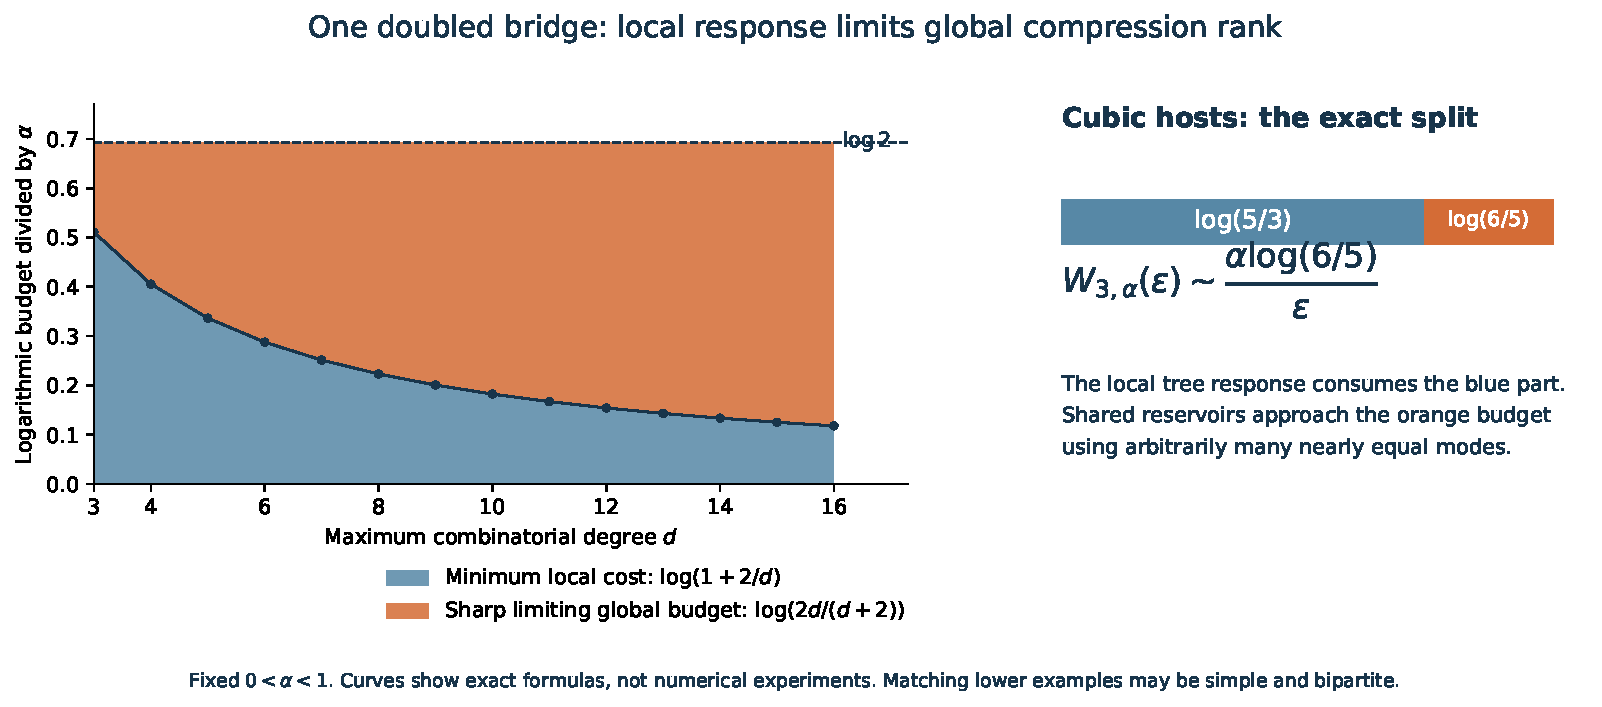
\includegraphics[width=\textwidth]{figures/local-global-bridge-budget.pdf}
\caption{For bridge edits, the regular-tree local response forces the
minimum local logarithmic budget shown in blue. The orange amount is the
sharp limiting budget available to arbitrarily many nearly equal global
modes. The formulas are exact; no finite-host spectral direct sum or
numerical convergence rate is asserted. The all-edge upper follows from
the separate free/wired comparison.}
\label{sharp:fig:budget}
\end{figure}

